\documentclass[a4paper,14pt,oneside]{extreport}

\usepackage{fontspec}           % Поддержка OpenType-шрифтов
\usepackage[russian]{babel}     % Поддержка русского языка
\setmainfont{Times New Roman}   % Times New Roman

\usepackage{setspace}           % Поддержка изменения интервала
\onehalfspacing                 % Полуторный интервал

\parindent=1.25cm               % Абзацный интервал
\usepackage{indentfirst}        % Отступ в первом абзаце раздела
\frenchspacing                  % Пробелы между предложениями = пробелам между словами

\tolerance=1                    % 
\emergencystretch=\maxdimen     % Не переносить слова
\hyphenpenalty=10000            %
\hbadness=10000                 %

\usepackage{geometry}           % 
\geometry{left=3cm}             %
\geometry{right=1.5cm}          % Поля
\geometry{top=2.0cm}            %
\geometry{bottom=2.0cm}         %


\setcounter{tocdepth}{2}        % Глубина оглавления до подпункта


\usepackage{graphicx}                  % Картинки
\graphicspath{ {./images/} }           % Директория с картинками
\setlength{\belowcaptionskip}{25pt}    % Отступ после картинки


\usepackage{amsmath}            % Перенос строки в уравнениях

\usepackage{pdfpages}           % Встраивание pdf               %

\makeatletter
\bibliographystyle{ugost2008}
\renewcommand{\@biblabel}[1]{#1.}
\makeatother

\begin{document}
    \includepdf[pages=-]{pdf/Титульный лист}
    \includepdf[pages=-]{pdf/Задание}
    \includepdf[pages=-]{pdf/Аннотация}
    
    \tableofcontents
    \newpage

    \chapter{Список терминов}

\parindent=0cm

Атрибут - специальный класс в C\#, позволяющий добавлять классам и их членам дополнительные метаданные

Вершина - позиция с дополнительной информацией, такой, как цвет, нормаль и UV-координата

Грань - замкнутое множество рёбер, чаще всего имеющее форму треугольника

Кватернион - гиперкомплексное число, образующее векторное пространство размерностью четыре над полем вещественных чисел и определяемое суммой $a + bi + cj + dk$, где $i$, $j$, $k$ - мнимые единицы, такие, что $i^{2} = j^{2} = k^{2} = ijk = -1$

Кривые Безье - тип параметрических кривых, описываемых с помощью опорных точек

Линейная интерполяция - функция, вычисляющая значение между $a$ и $b$ на основе приращения $t$

Материал - описание визуальных свойств модели, например, отражающей способности, используемых шейдеров и текстур

Префаб - специальный тип ассетов Unity, позволяющий хранить объект вместе со всеми компонентами и значениями свойств

Полигон - набор граней, лежащих в одной плоскости

Полигональная сетка - совокупность вершин, рёбер и граней, определяющих форму объекта

Процедурная генерация - программная генерация контента с использованием специальных алгоритмов

Ребро - соединение между двумя вершинами

Сериализация - сохранение структуры данных в виде последовательности битов

Текстура - плоское изображение, накладываемое на полигональную сетку

Трёхмерная модель - изображение объекта в трёхмерном пространстве

Шейдер - программа, испольняемая видеокартой

C\# - объектно-ориентированный язык программирования, используемый для написания скриптов и расширений для редактора в Unity

L-системы - вид формальных грамматик, основанный на переписывании строки

Low poly - минималистичный стиль графики, использующий сравнительно низкое число полигонов и раскраску вершин

Unity - кроссплатформенный игровой движок, поддерживающий более 25 платформ

UV-координаты - отображение координат вершин на координаты текстуры

\parindent=1.25cm

    \chapter{Введение}

В мультимедиа и в частности в играх широко применяется процедурная генерация, использующая специальные алгоритмы для создания контента самостоятельно или при взаимодействии с разработчиками. Процедурная генерация может применяться для генерации уровней, объектов, персонажей, квестов, текстур, анимации и многого другого. Целью использования процедурной генерации может быть повышение реиграбельности и ускорение создания разнообразного контента.

Одним из первых примеров игр, применяющих процедурную генерацию контента, является Rogue. В этой ролевой игре 1980 года игрок брал на себя роль искателя приключений, исследующего процедурно сгенерированное подземелье. \cite{Rogue} Rogue породила целый жанр игр, названный в её честь - roguelike. В таких играх большая часть контента, включая уровни, предметы и противников, генерируется процедурно.

Процедурная генерация также применяется для генерации графики. В частности, возможно применять её для генерации внутриигровых объектов, чтобы упростить работу разработчикам и освободить время на работу над геймплеем и сценарием. 

Деревья являются одной из самых распространённых декораций в видеоиграх. Они используются часто и в большом количестве, но при этом являются лишь второстепенной частью окружения, а следовательно, неудачно сгенерированное дерево практически не влияет на погружение. В силу этих причин имеет смысл генерировать деревья процедурно, чтобы обеспечить вариативность, делая локации более правдоподобными и упрощая ориентирование по ним. 

Ярким примером программного обеспечения для процедурной генерации растительности является система SpeedTree, выпущенная в 2002 году. С тех пор SpeedTree была использована для генерации деревьев в многочисленных играх крупнейших студий, например, Bethesda Softworks, Ubisoft и CD Projekt Red. SpeedTree широко используется в фильмах, начиная с <<Аватара>> Джеймса Кэмерона, вышедшего в 2009 году. Помимо этого, она используется в различных приложениях-симуляторах, к примеру, в симуляторе лесных пожаров, разработанном в Университете Центральной Флориды.

Для процедурной генерации моделей растительности в большинстве случаев применяются системы Линденмайера, или L-системы. L-система - это вид формальной грамматики, изначально предназначенный для моделирования процесса развития растения. Их рекурсивная природа приводит к самоподобию, позволяя описывать подобные фракталам органические формы. Таким образом можно получить сложные, детализированные и реалистичные модели.

Однако деревья, сгенерированные с помощью систем наподобие SpeedTree, подходят лишь для проектов с реалистичной и детализированной графикой. Независимые разработчики зачастую используют стилизованную графику в стиле low poly - техники, в которой используется сравнительно небольшое число полигонов. Такой стиль обладает рядом преимуществ по сравнению с реалистичной графикой, наиболее важное из которых - низкий порог вхождения. Поскольку модели построены на графических примитивах, создавать их может даже программист без способностей к рисованию и моделированию. При небольшом количестве полигонов можно создавать достаточно красивые модели без использования текстур, используя раскраску вершин. По этим причинам low poly снижает стоимость разработки проекта, освобождая время и ресурсы. Кроме того, низкополигональные модели отличаются более высокой скоростью загрузки и сниженными требованиями к аппаратному обеспечению по сравнению с высокополигональными, что особенно важно на мобильных платформах. \cite{LowPolyIntro} 

В рамках данной работы будет разработан плагин для движка Unity 3D, позволяющий генерировать стилизованные низкополигональные модели деревьев, подходящие для использования в качестве внутриигровых объектов. Деревья можно будет генерировать как непосредственно в игре, так и заранее. Для генерации дерева необходимо добавить к игровому объекту специальный скрипт, позволяющий настроить параметры. Для создания предустановок можно использовать систему префабов Unity.
 
\newpage

    \chapter{Обзор аналогов}
\section{SpeedTree}
\subsection{История}
SpeedTree - комплекс программных продуктов, разрабатываемый компанией Interactive Data Visualisation. 

Первая версия SpeedTree называлась SpeedTreeCAD и была создана IDV в 2000 году для использования в симуляторе гольфа. Позже CAD был преобразован в плагин для 3D Studio Max (ныне Autodesk 3ds Max) под названием SpeedTreeMax. 

В конце 2002 года IDV выпустила SpeedTreeRT - SDK для рендеринга деревьев в реальном времени. SpeedTreeRT поддерживал несколько уровней детализации, эффект ветра и различные уровни освещения. Также был разработан SpeedTreeMAYA - аналогичный SpeedTreeMax плагин для Maya. 

В 2009 году разработка этих плагинов была завершена, и им на смену пришёл SpeedTree 5. В его состав вошли три компонента: редактор SpeedTree Modeler, SpeedTreeSDK и SpeedTree Compiler, предназначенный для подготовки файлов SpeedTree к рендерингу в реальном времени. 

\subsection{Состав}
В настоящее время SpeedTree включает в себя следующие программные комплекты:
\subsubsection{SpeedTree Cinema}
SpeedTree Cinema - комплект программного обеспечения, предназначенный для использования в кинематографе. Он был выпущен в 2009 и с тех широко используется для генерации деревьев в фильмах, начиная с ``Аватара'' Джеймса Кэмерона. SpeedTree Cinema генерирует полигональные сетки и текстуры высокого разрешения для различных редакторов трёхмерной графики.

\subsubsection{SpeedTree Studio}
SpeedTree Studio является бюджетной версией SpeedTree Cinema. Он включает в себя подмножество возможностей этого комплекта.

\subsubsection{SpeedTree Architect}
SpeedTree Architect предназначен для экспорта моделей в CAD, такие, как Maya и Autodesk 3ds Max.

\subsubsection{SpeedTree for Games}
SpeedTree for Games - издание, предназначенное для разработки игр. Оно включает в себя Modeler, Compiler и SDK и может быть интегрировано в любой игровой движок. Сгенерированные полигональные сетки отличаются большей оптимизацией по сравнению с другими изданиями SpeedTree.

\subsubsection{SpeedTree Subscription Edition}
SpeedTree Subscription Edition - бюджетное решение, рассчитанное на независимых разработчиков игр. Подписка на этот продукт даёт доступ к редактору и генерации деревьев и растений. Полученные модели могут быть использованы только в Unity или Unreal Engine, в зависимости от приобретённой лицензии. Также за дополнительную плату можно приобрести комплекты готовых моделей из библиотеки.

\begin{figure}[h]
    \centering
    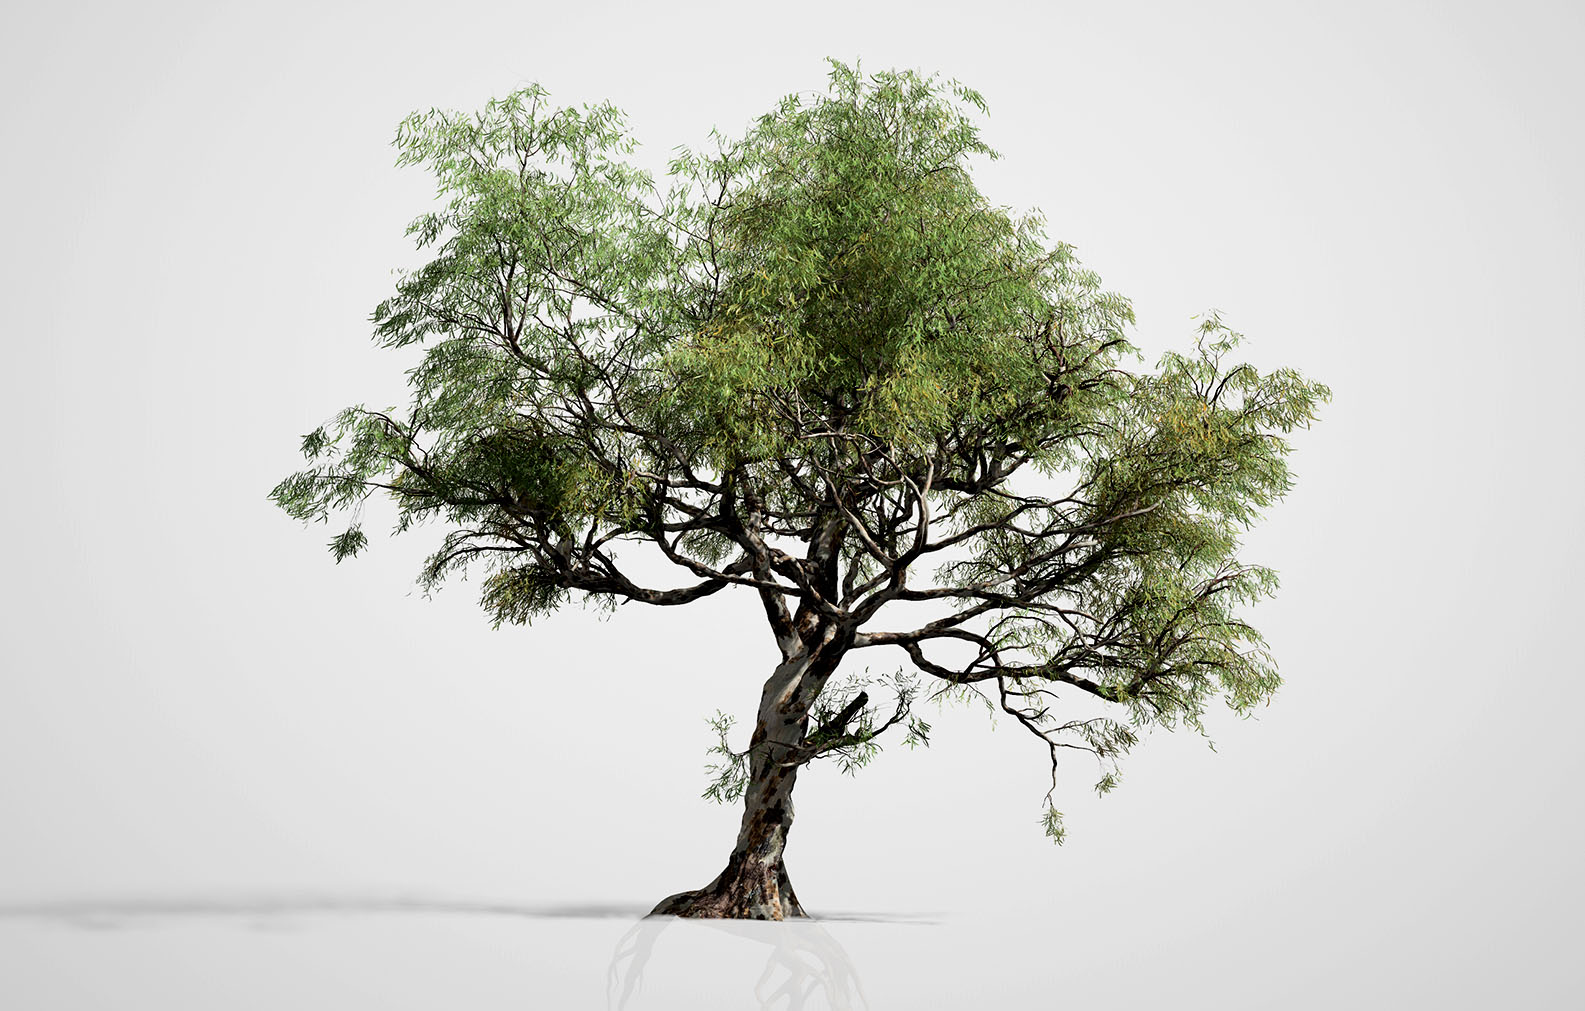
\includegraphics[width=0.8\textwidth]{speedtree}
    \caption{Пример дерева, сгенерированного при помощи SpeedTree.}
\end{figure}

\section{TreeIt}
TreeIt - бесплатное программное обеспечение для генерации растительности, разработанное Evolved Software для Microsoft Windows. TreeIt позволяет создавать высококачественные модели растений различных видов, включая не только деревья, но также кактусы и цветы.

Поддерживается экспорт в форматы dbo, obj, fbx и x. Присутствует возможность регуляции уровня детализации. Все модели, сгенерированные при помощи TreeIt, абсолютно бесплатны для использования в любых проектах.

\begin{figure}[h]
    \centering
    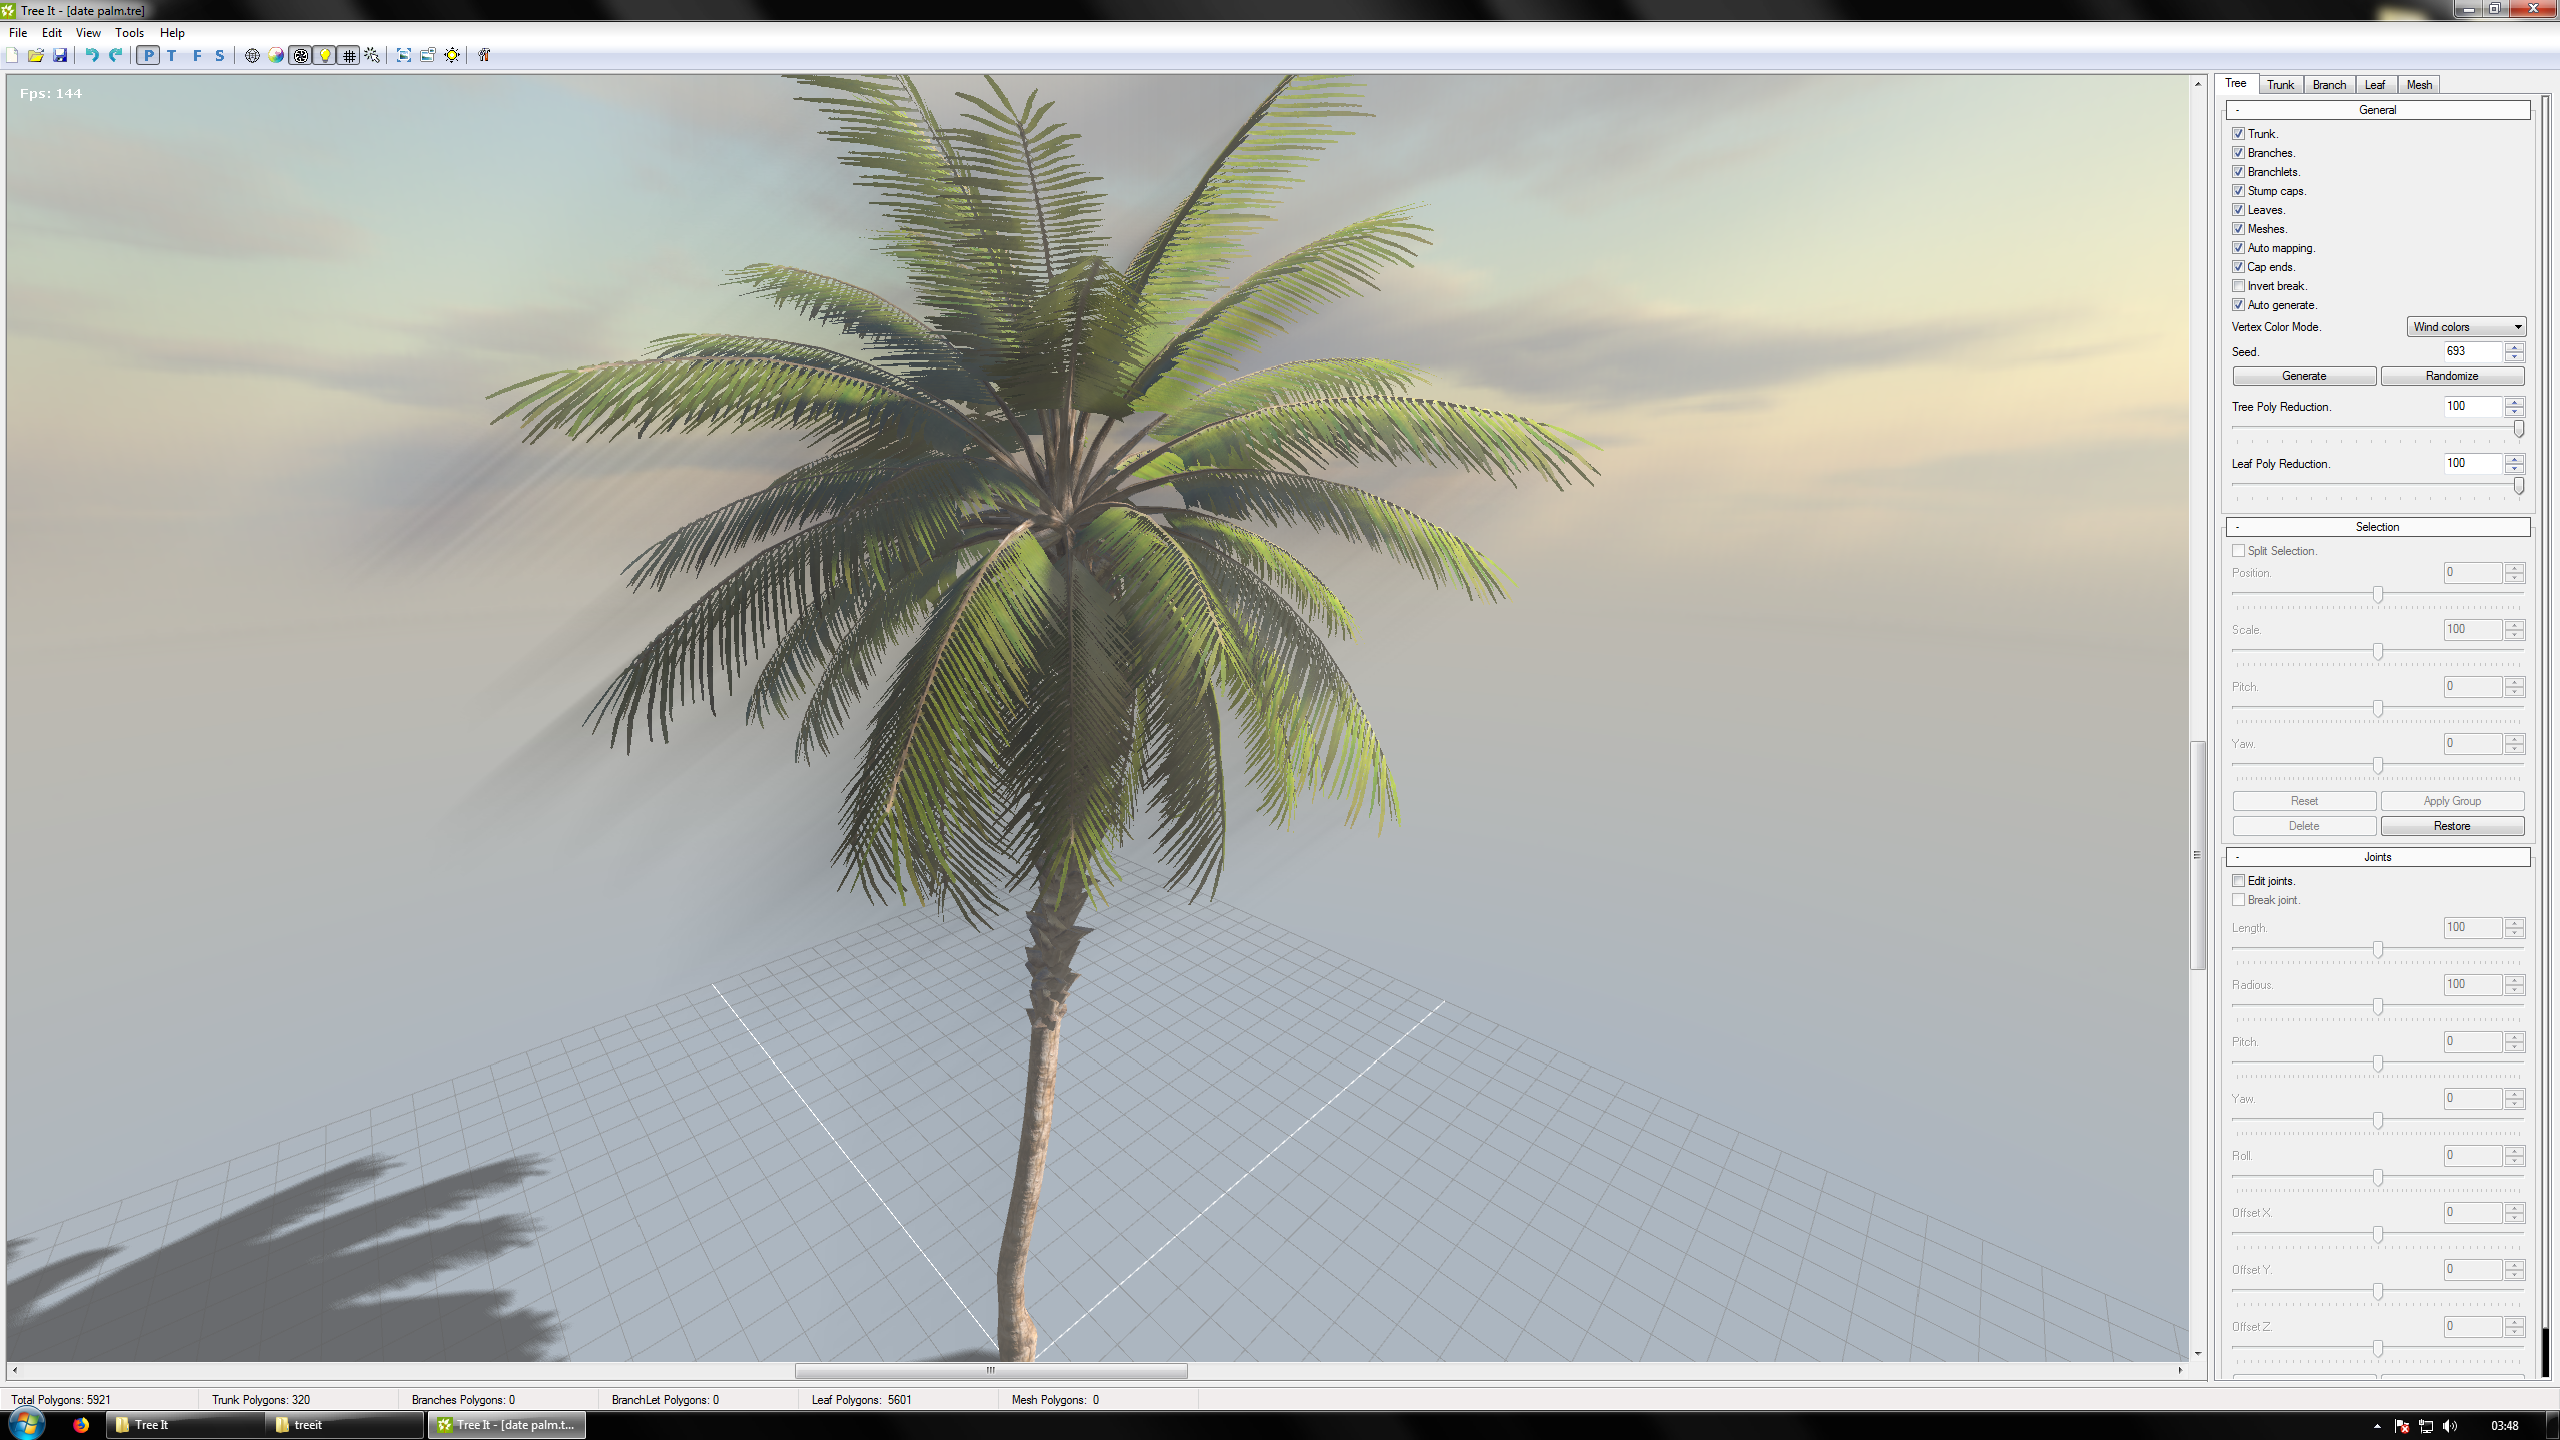
\includegraphics[width=0.8\textwidth]{treeit}
    \caption{Пример дерева, сгенерированного при помощи TreeIt.}
\end{figure}

\newpage
\section{TreeGen}
TreeGen - плагин для генерации деревьев в редакторе трёхмерных моделей Blender, распространяемый свободно по лицензии MIT.

TreeGen использует комбинацию из двух подходов: системы Линденмайера и параметрический подход.

\begin{figure}[h]
    \centering
    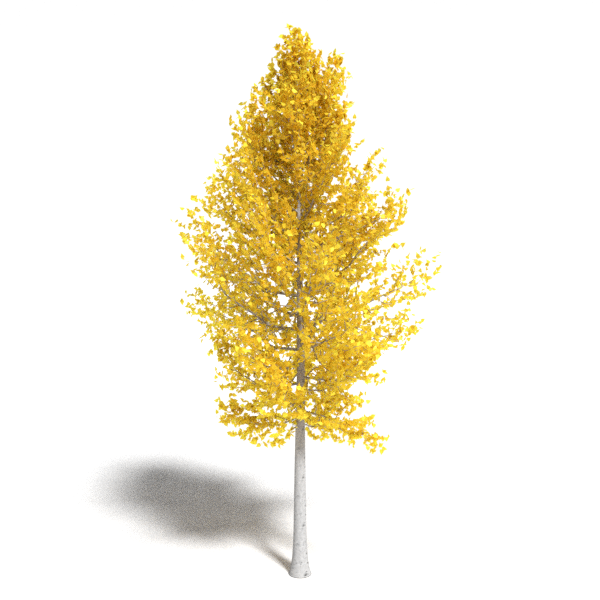
\includegraphics[width=0.8\textwidth]{treegen}
    \caption{Пример дерева, сгенерированного в плагине Treegen.}
\end{figure}

\section{Unity Tree Creator}

\newpage

    \chapter{Теоретическая часть и проектирование}
\section{Выбор движка}
Было принято решение использовать в качестве платформы игровой движок \emph{Unity}. Unity широко используется в компьютерных, консольных и мобильных играх, а также в приложениях дополненной и виртуальной реальности. Этот движок используется как крупными компаниями, так и независимыми разработчиками.

Главное преимущество игрового движка перед специализированным программным обеспечением для трёхмерного моделирования - это возможность генерировать деревья непосредственно в игре. Такой подход позволяет делать каждое дерево уникальным, что немаловажно при процедурной генерации уровней. Кроме того, отпадает необходимость экспорта и загрузки десятков разных моделей; для создания дерева достаточно прикрепить нужный компонент к игровому объекту. 

\section{Выбор стиля}
В качестве графического стиля был выбран \emph{low poly} - стиль, в котором намеренно используется низкое число полигонов для достижения угловатого и минималистичного внешнего вида. Как было сказано во введении, подобные модели строятся из геометрических примитивов и зачастую не используют текстуры, благодаря чему их гораздо проще создавать по сравнению с высокополигональными моделями. По тем же причинам они хорошо подходят для процедурной генерации. 

На рисунке ~\ref{fig:lowpoly} изображены модели деревьев, выполненные в этом стиле.

\begin{figure}[h]
    \centering
    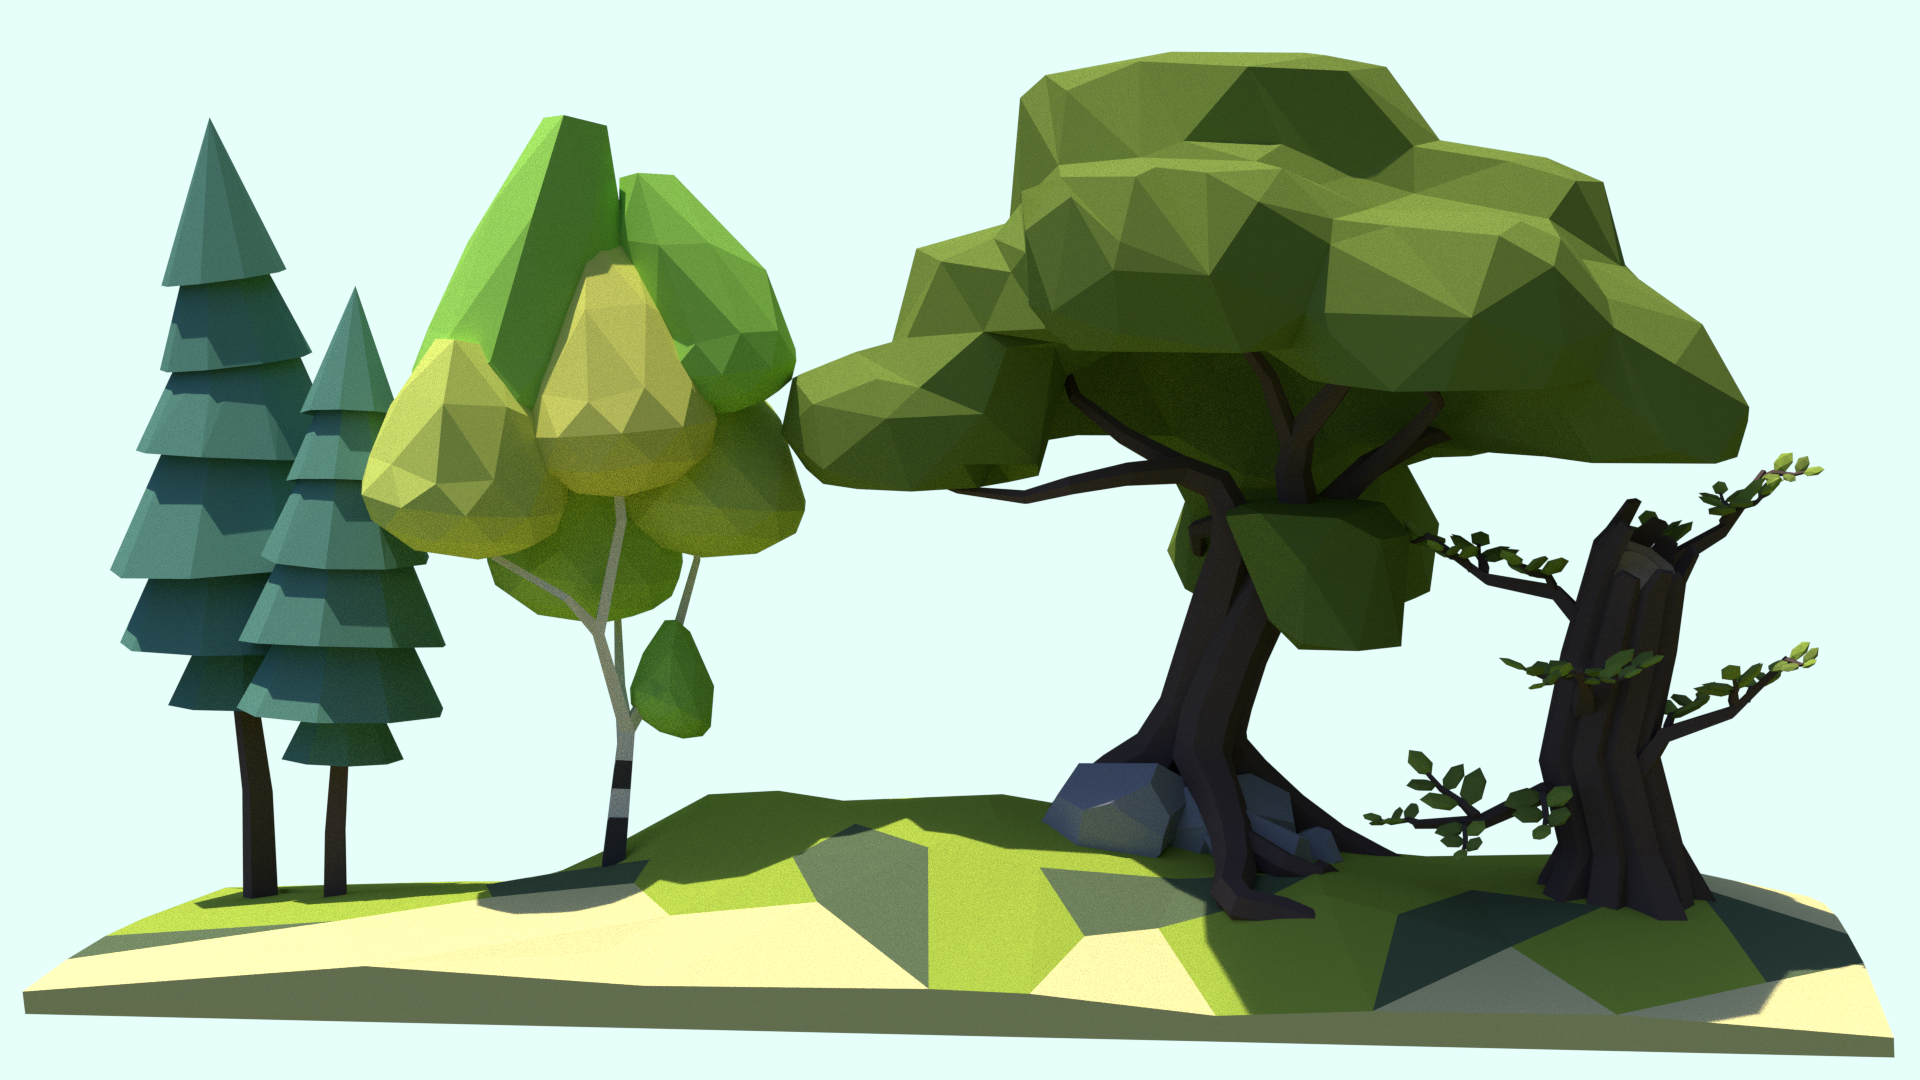
\includegraphics[width=0.8\textwidth]{lowpoly}
    \caption{Деревья в стиле Low poly. Автор: Lars Mezaka}
    \label{fig:lowpoly}
\end{figure}

Важной составляющей low poly является уровень детализации. Он должен поддерживаться на постоянном уровне. К примеру, если имеется модель камня и необходима модель камня меньшего размера, то использовать уменьшенную модель большого камня нежелательно, поскольку в этом случае маленький камень получится более детализированным и не будет сочетаться с остальной сценой визуально. Вместо этого лучше создать для него отдельную модель. Исходя из этого принципа, уровень детализации сгенерированных моделей будет выбираться автоматически в зависимости от параметров. К примеру, в стволе тонкого дерева будет меньше граней, чем в стволе более толстого.

\section{Описание движка Unity}
Unity - кроссплатформенный игровой движок, впервые выпущенный в 2005 году американской компанией Unity Technologies. В Unity применяется модульная система компонентов, позволяющая добавлять объектам необходимый функционал с помощью Drag-and-drop интерфейса. Для написания скриптов используется язык программирования C\#, работающий на свободной и кроссплатформенной реализации платформы .NET - Mono.

Ключевые особенности Unity - это наличие визуального редактора с множеством полезных инструментов для разработки и отладки приложений, возможность быстрого создания прототипов и поддержка более 25 платформ. Unity имеет несколько лицензий, одна из которых бесплатна и может использоваться при условии, что ежегодный доход от продажи игры не превышает 100000 долларов США. Редактор доступен для Windows и MacOS; с 2019 года доступна экспериментальная версия для Linux в независимом от дистрибутива формате AppImage.

\section{Структура 3D-модели}
Термины ``3D model'' (трёхмерная модель) и ``mesh'' (полигональная сетка) часто путают и используют как синонимы. Разница в том, что полигональная сетка содержит только информацию о геометрии, а модель, помимо полигональной сетки, может содержать и другую информацию, к примеру, анимацию или текстуры.

\emph{Полигональная сетка} - это совокупность вершин, рёбер и граней, которая определяет форму объекта. Помимо этого, полигональная сетка может содержать данные о нормалях, касательных, цветах вершин и \emph{UV-координатах}, которые применяются для наложения текстуры на сетку.

\emph{Грани} в трёхмерной графике являются многоугольниками. Чаще всего они имеют форму треугольника, потому что треугольник гарантированно лежит в одной плоскости, и благодаря этому свойству их проще обрабатывать и отрисовывать. 

Грани описываются \emph{массивом индексов вершин}, из которых они состоят. Зачем описывать вершины и грани по отдельности, если грань можно описать координатами вершин? Преимущество такого подхода в уменьшении использования памяти. Поскольку у смежных граней всегда будут общие вершины, дублирование данных в массиве неизбежно; однако при использовании индексов необходимо дублировать лишь 32 бита против 96 битов трёхмерного вектора, задающего вершину.

\section{Средства работы с полигональными сетками в Unity}
Трёхмерная модель в Unity представлена классом \texttt{Mesh}\cite{UnityMesh}. Его основные наборы данных - это массив вершин и массив треугольников.

Массив треугольников содержит тройки индексов вершин, образующих треугольник. Важной особенностью является то, что треугольник отрисовывается только в том случае, если порядок обхода вершин в проекции треугольника на экран соответствует обходу по часовой стрелке. Это правило удовлетворяет конвенции OpenGL и оптимизирует рендеринг, позволяя отсекать лишние грани, направленные против камеры.

Также \texttt{Mesh} содержит необязательные наборы данных. Нормали и касательные используются для расчёта освещения и могут быть посчитаны автоматически. UV-координаты в данной работе не затрагиваются, поскольку не используются текстуры.

Для управления моделями игровых объектов в Unity существует несколько компонентов. \emph{Mesh Filter} - это контейнер для модели, который предоставляет к ней доступ для других компонентов. \emph{Mesh Renderer} отвечает за освещение и рендеринг модели и предоставляет доступ к \emph{материалу} (материалам). Материал - это описание визуальных свойств модели. Он включает в себя описание отражающей способности, шейдеров и текстур, а также некоторых других свойств.
\newpage

    \chapter{Разработка}
\section{Рендеринг}
Прежде чем приступать к созданию генератора, было необходимо подобрать шейдер для отрисовки моделей. Этот шейдер должен поддерживать цветные вершины и \emph{плоское освещение}, то есть такое освещение, при котором цвет вычисляется не для каждой отдельной вершины, а для целых граней. Такое освещение применяется в стиле low poly для создания стилизованного изображения. 

\begin{figure}[h]
    \centering
    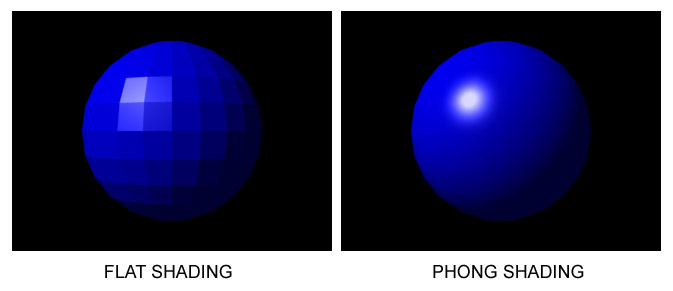
\includegraphics[width=\textwidth]{phong}
    \caption{Плоское освещение и освещение по Фонгу.}
\end{figure}

Для демонстрационных целей в работе был использован шейдер, взятый из блога Hextant Studios\cite{FlatShader}. Результирующий плагин будет независим от конкретного шейдера, и в нём будет реализована поддержка отдельных материалов для листьев и ствола.



\section{Генерация листьев}
Разработка была начата с генератора \emph{круглой листвы}. Для этого были изучены руководства по моделированию в стиле low poly, чтобы максимально приблизить программную реализацию генератора к тому, как моделирует человек.

Генерация листьев проходит в несколько шагов:
\begin{enumerate}
\item Генерируется модель икосаэдра радиусом в одну единицу. У икосаэдра 12 вершин с координатами 
(\texttt{\(0, \pm\Phi, \pm1\)}), 
(\texttt{\(\pm1, 0, \pm\Phi\)}), 
(\texttt{\(\pm\Phi, \pm1, 0\)}) и 20 треугольных граней.\cite{IcosahedronMath}
Векторы вершин нормализуются, чтобы привести радиус фигуры к единице. Также фигура поворачивается на случайный угол.

Для описания поворотов в трёхмерном пространстве в компьютерной графике широко применяются \emph{кватернионы}. Кватернион - это гиперкомплексное число, образующее векторное пространство размерностью четыре над полем вещественных чисел, которое можно представить как сумму вида

\begin{equation}
    q = a + bi + cj + dk,
\end{equation}

где $i$, $i$, $k$ - мнимые единицы, такие, что $i^2 = j^2 = k^2 = ijk = -1$. Свойства кватернионов делают их удобным инструментом для описания вращения\cite{quaternions}.

В Unity кватернионы представлены классом \texttt{Quaternion}. Для получения случайного поворота существует свойство \texttt{Random.rotation}. Кватернион умножается на вектор для поворота последнего, причём операция не ассоциативна и кватернион должен быть первым операндом, а вектор - вторым. Таким образом, чтобы повернуть модель, надо умножить кватернион на каждую её вершину.

\item Для увеличения количества граней применяется \emph{алгоритм подразделения}\cite{Subdivision}, который применяется для создания икосфер. Икосфера - это приближённый к сфере многогранник, полученный путём разделения каждой грани на четыре и последующего смещения новых вершин на поверхность описанной сферы. На рисунке ~\ref{fig:subdivision} показан пример икосферы, полученной с использованием двух итераций подразделения.
 
\begin{figure}[h]
    \centering
    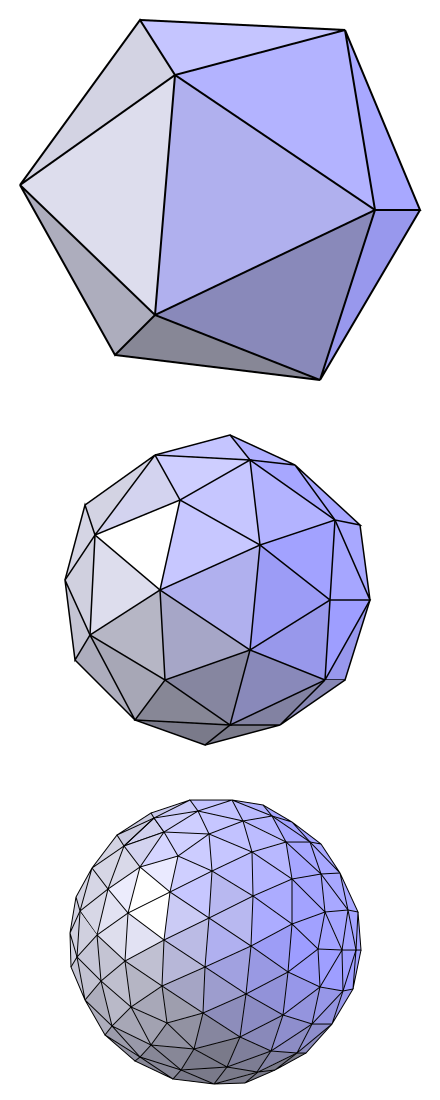
\includegraphics[height=0.5\textwidth, angle=90]{subdivision}
    \caption{Пример двукратного подразделения икосаэдра. Автор: Simon Fuhrmann, Wikimedia}
    \label{fig:subdivision}
\end{figure}

В нашем случае достаточно всего одной итерации подразделения, которая повысит число полигонов с 20 до 80. Поскольку уровень детализации определяется автоматически, было решено использовать подразделение только для листвы, ширина или высота которой не меньше значения по умолчанию (3 единицы).

Блок-схема алгоритма подразделения приведена на рисунке ~\ref{fig:subdivisionFlowchart}.

\begin{figure}[h]
    \centering
    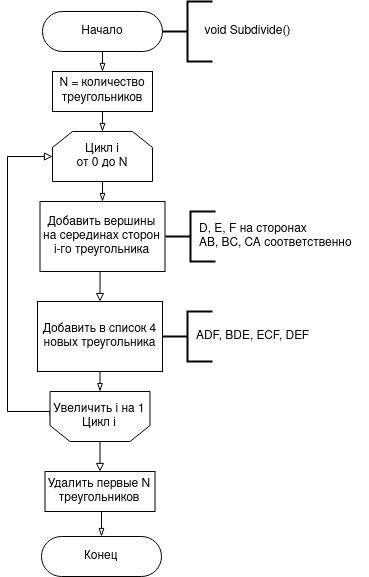
\includegraphics[width=0.6\textwidth]{subdivisionFlowchart}
    \caption{Блок-схема алгоритма подразделения.}
    \label{fig:subdivisionFlowchart}
\end{figure}

\item Фигура растягивается для достижения заданной ширины и высоты. Для каждой вершины вычисляется радиус (то есть длина вектора) по следующей формуле:

\begin{equation}
    r = lerp\left(width, height, \frac{\left|y_{v}\right|}{|v|}\right),
\end{equation}

где $lerp$ - функция линейной интерполяции, 

$width$ и $height$ - заданные ширина и высота листвы,

$v$ - вектор, задающий вершину.

\item Наконец, вершины случайным образом смещаются для придания листве более натурального вида. Однако если две вершины поменяются местами, то геометрия листвы будет нарушена, поскольку грани начнут пересекаться. Следовательно, для каждой вершины необходимо найти максимальный допустимый радиус смещения, при котором многогранник сохранит правильную форму.

Для нахождения максимального допустимого смещения используется следующая формула:

\begin{equation}
    maxshift_{i} = \frac{\displaystyle\min_{j = 0}^n(|V_{i} - N^{i}_{j}|)}{3}, 
\end{equation}
где $V$ - множество всех вершин, 

$N^{i}$ - множество соседей текущей вершины, 

$n$ - общее число соседей.

Полученное значение умножается на случайное значение от 0 до 1 и случайный единичный вектор, чтобы получить итоговое смещение для этой вершины.

Блок-схема алгоритма смещения вершин приведена на рисунке ~\ref{fig:displacementFlowchart}. 

\end{enumerate}

На рисунке ~\ref{fig:leaves} изображён пример листвы, сгенерированной с использованием вышеописанных алгоритмов.

\begin{figure}[h]
    \centering
    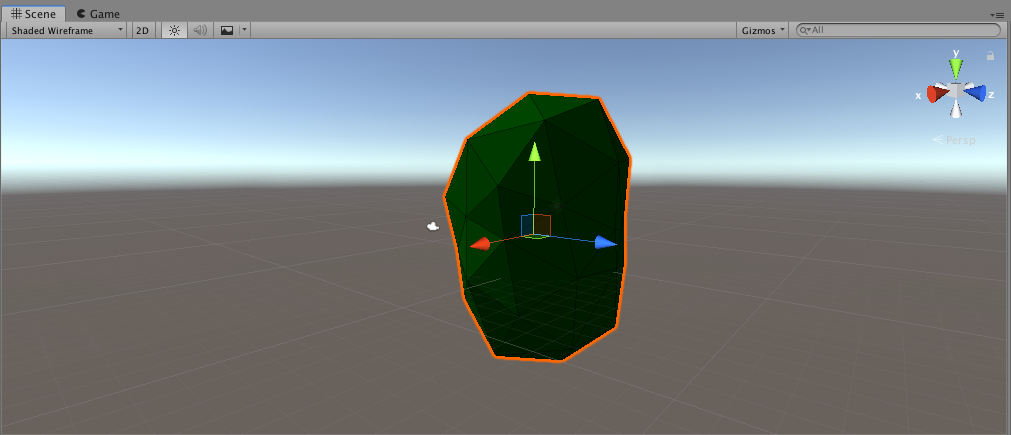
\includegraphics[width=0.8\textwidth]{leaves}
    \caption{Процедурно сгенерированная листва.}
    \label{fig:leaves}
\end{figure}



\begin{figure}[h]
    \centering
    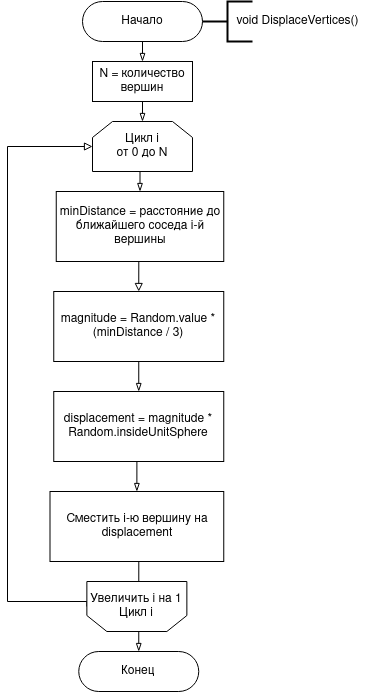
\includegraphics[width=0.5\textwidth]{displacementFlowchart}
    \caption{Блок-схема алгоритма смещения вершин.}
    \label{fig:displacementFlowchart}
\end{figure}

\section{Генерация ствола}
На первых этапах разработки генератора стволов был рассмотрен схожий проект\cite{hassank} на Github, посвящённый анимации роста процедурно генерируемых деревьев. Этот проект был заброшен на ранней стадии разработки, но алгоритм генерации ствола, используемый в нём, оказался полезен в данной работе; он был доработан и усовершенствован.

Ствол представляет собой пирамиду, разделённую на ярусы. Каждый ярус случайным образом поворачивается, задавая изгибы ствола. На конце ствола с помощью вышеописанного алгоритма генерируется крона, выделенная в отдельный игровой объект. Ствол состоит из 3-8 сегментов, количество которых пропорционально высоте.

На стволе также могут генерироваться ветви. С определённой вероятностью происходит выбор грани на текущем уровне, из которого может вырасти ветвь. Это возможно при условии, что высота текущего уровня не меньше 33\% от высоты дерева и не больше 90\%; это произвольно выбранные значения, предотвращающие генерацию ветвей в плохо подходящих для этого частях дерева. 

Второе условие генерации ветви заключается в том, что выбранная на уровне грань не должна быть направлена вниз, потому что ветвь не может расти вниз. Таким образом, нормаль выбранной грани должна иметь положительную компоненту по вертикальной оси. Также ветви не растут на деревьях с плоской листвой и хвоей.

Если эти условия выполнены, то создаётся объект генератора ветви и помещается в список, который будет обработан в последнюю очередь. Такое решение было принято для того, чтобы не нарушать порядок вершин, использованных в стволе. Ветвь начинает расти перпендикулярно стволу, но постепенно поворачивается вертикально вверх. 

Кроме того, с определённой вероятностью дерево может оказаться пнём. В таком случае оно будет обрублено в случайном месте. На срубе будет видна древесина и обломки коры. Пример такого пня представлен на рисунке ~\ref{fig:stumpResult}.

\begin{figure}[!htb]
    \centering
    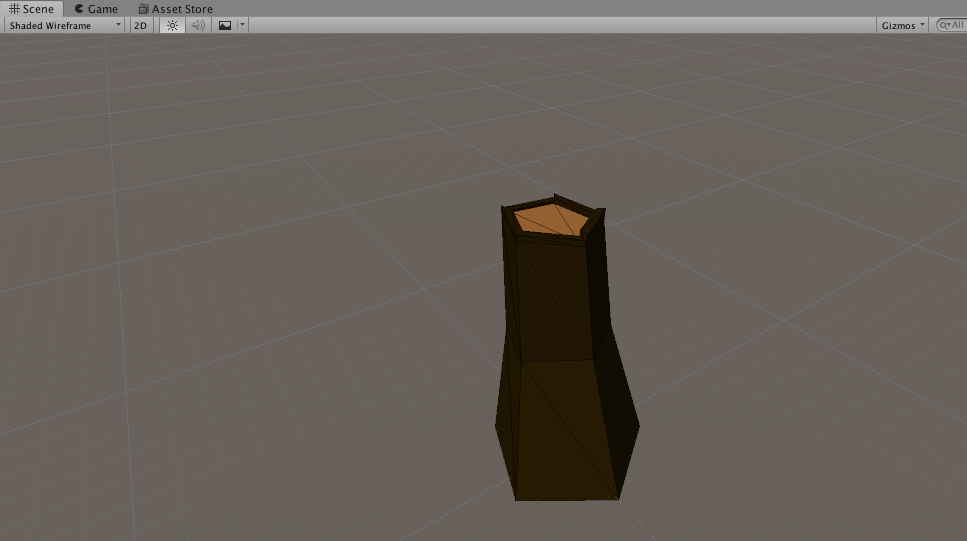
\includegraphics[width=0.8\textwidth]{stumpResult}
    \caption{Пример процедурно сгенерированного пня.}
    \label{fig:stumpResult}
\end{figure}

Блок-схема полного алгоритма генерации ствола приведена на рисунке ~\ref{fig:trunkFlowchart}.

На рисунке ~\ref{fig:roundResult} изображён пример процедурно сгенерированного дерева с круглой листвой.

\begin{figure}[!htb]
    \centering
    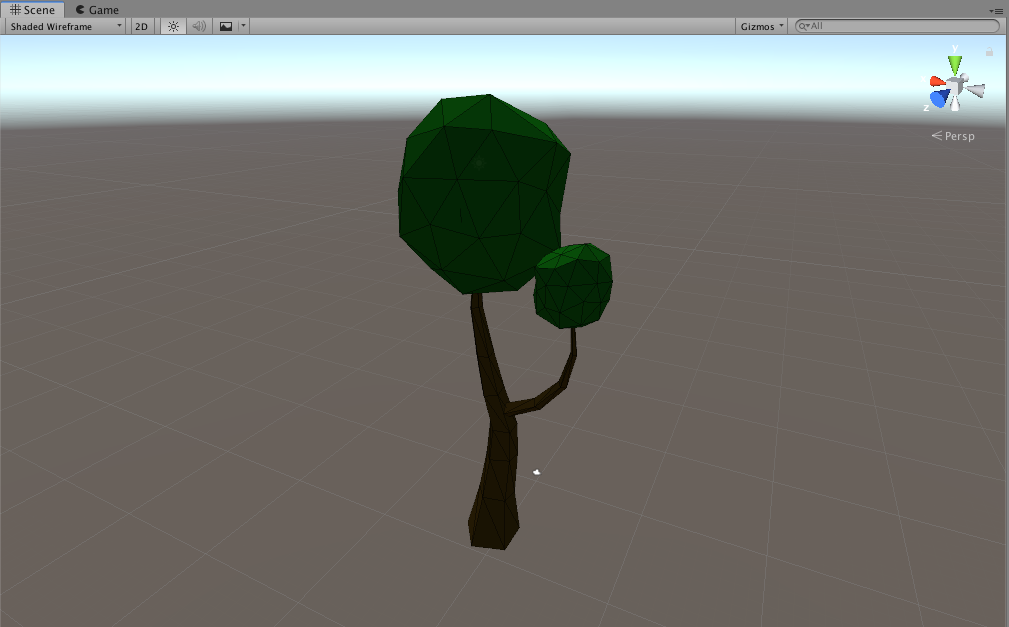
\includegraphics[width=0.8\textwidth]{roundResult}
    \caption{Пример процедурно сгенерированного дерева с круглой листвой.}
    \label{fig:roundResult}
\end{figure}

\begin{figure}[!htb]
    \centering
    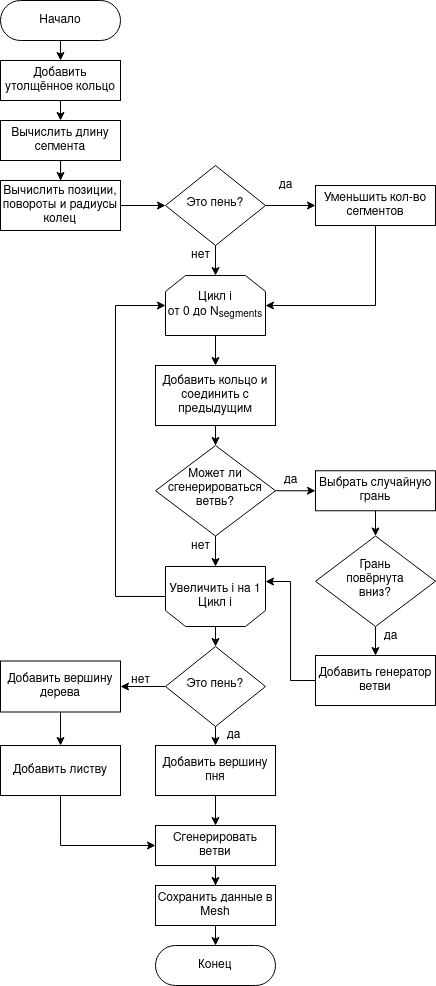
\includegraphics[width=0.6\textwidth]{trunkFlowchart}
    \caption{Блок-схема генерации ствола.}
    \label{fig:trunkFlowchart}
\end{figure}

\section{Генерация плоской листвы}
Разработанное расширение для редактора позволило ввести новые типы листьев, первым из которых стали \emph{плоские листья}, основанные на листьях пальм и древовидных папоротников. В реальности листья пальм имеют перистую либо веерную структуру, однако в силу минимализма графики в low poly для изображения пальмового листа обычно используют простую цепочку из полигонов. Иногда на её стороны добавляются ``насечки'', символизирующие перья. На рисунке ~\ref{fig:palmExample} изображена пальма в стиле low poly.

\begin{figure}[!htb]
    \centering
    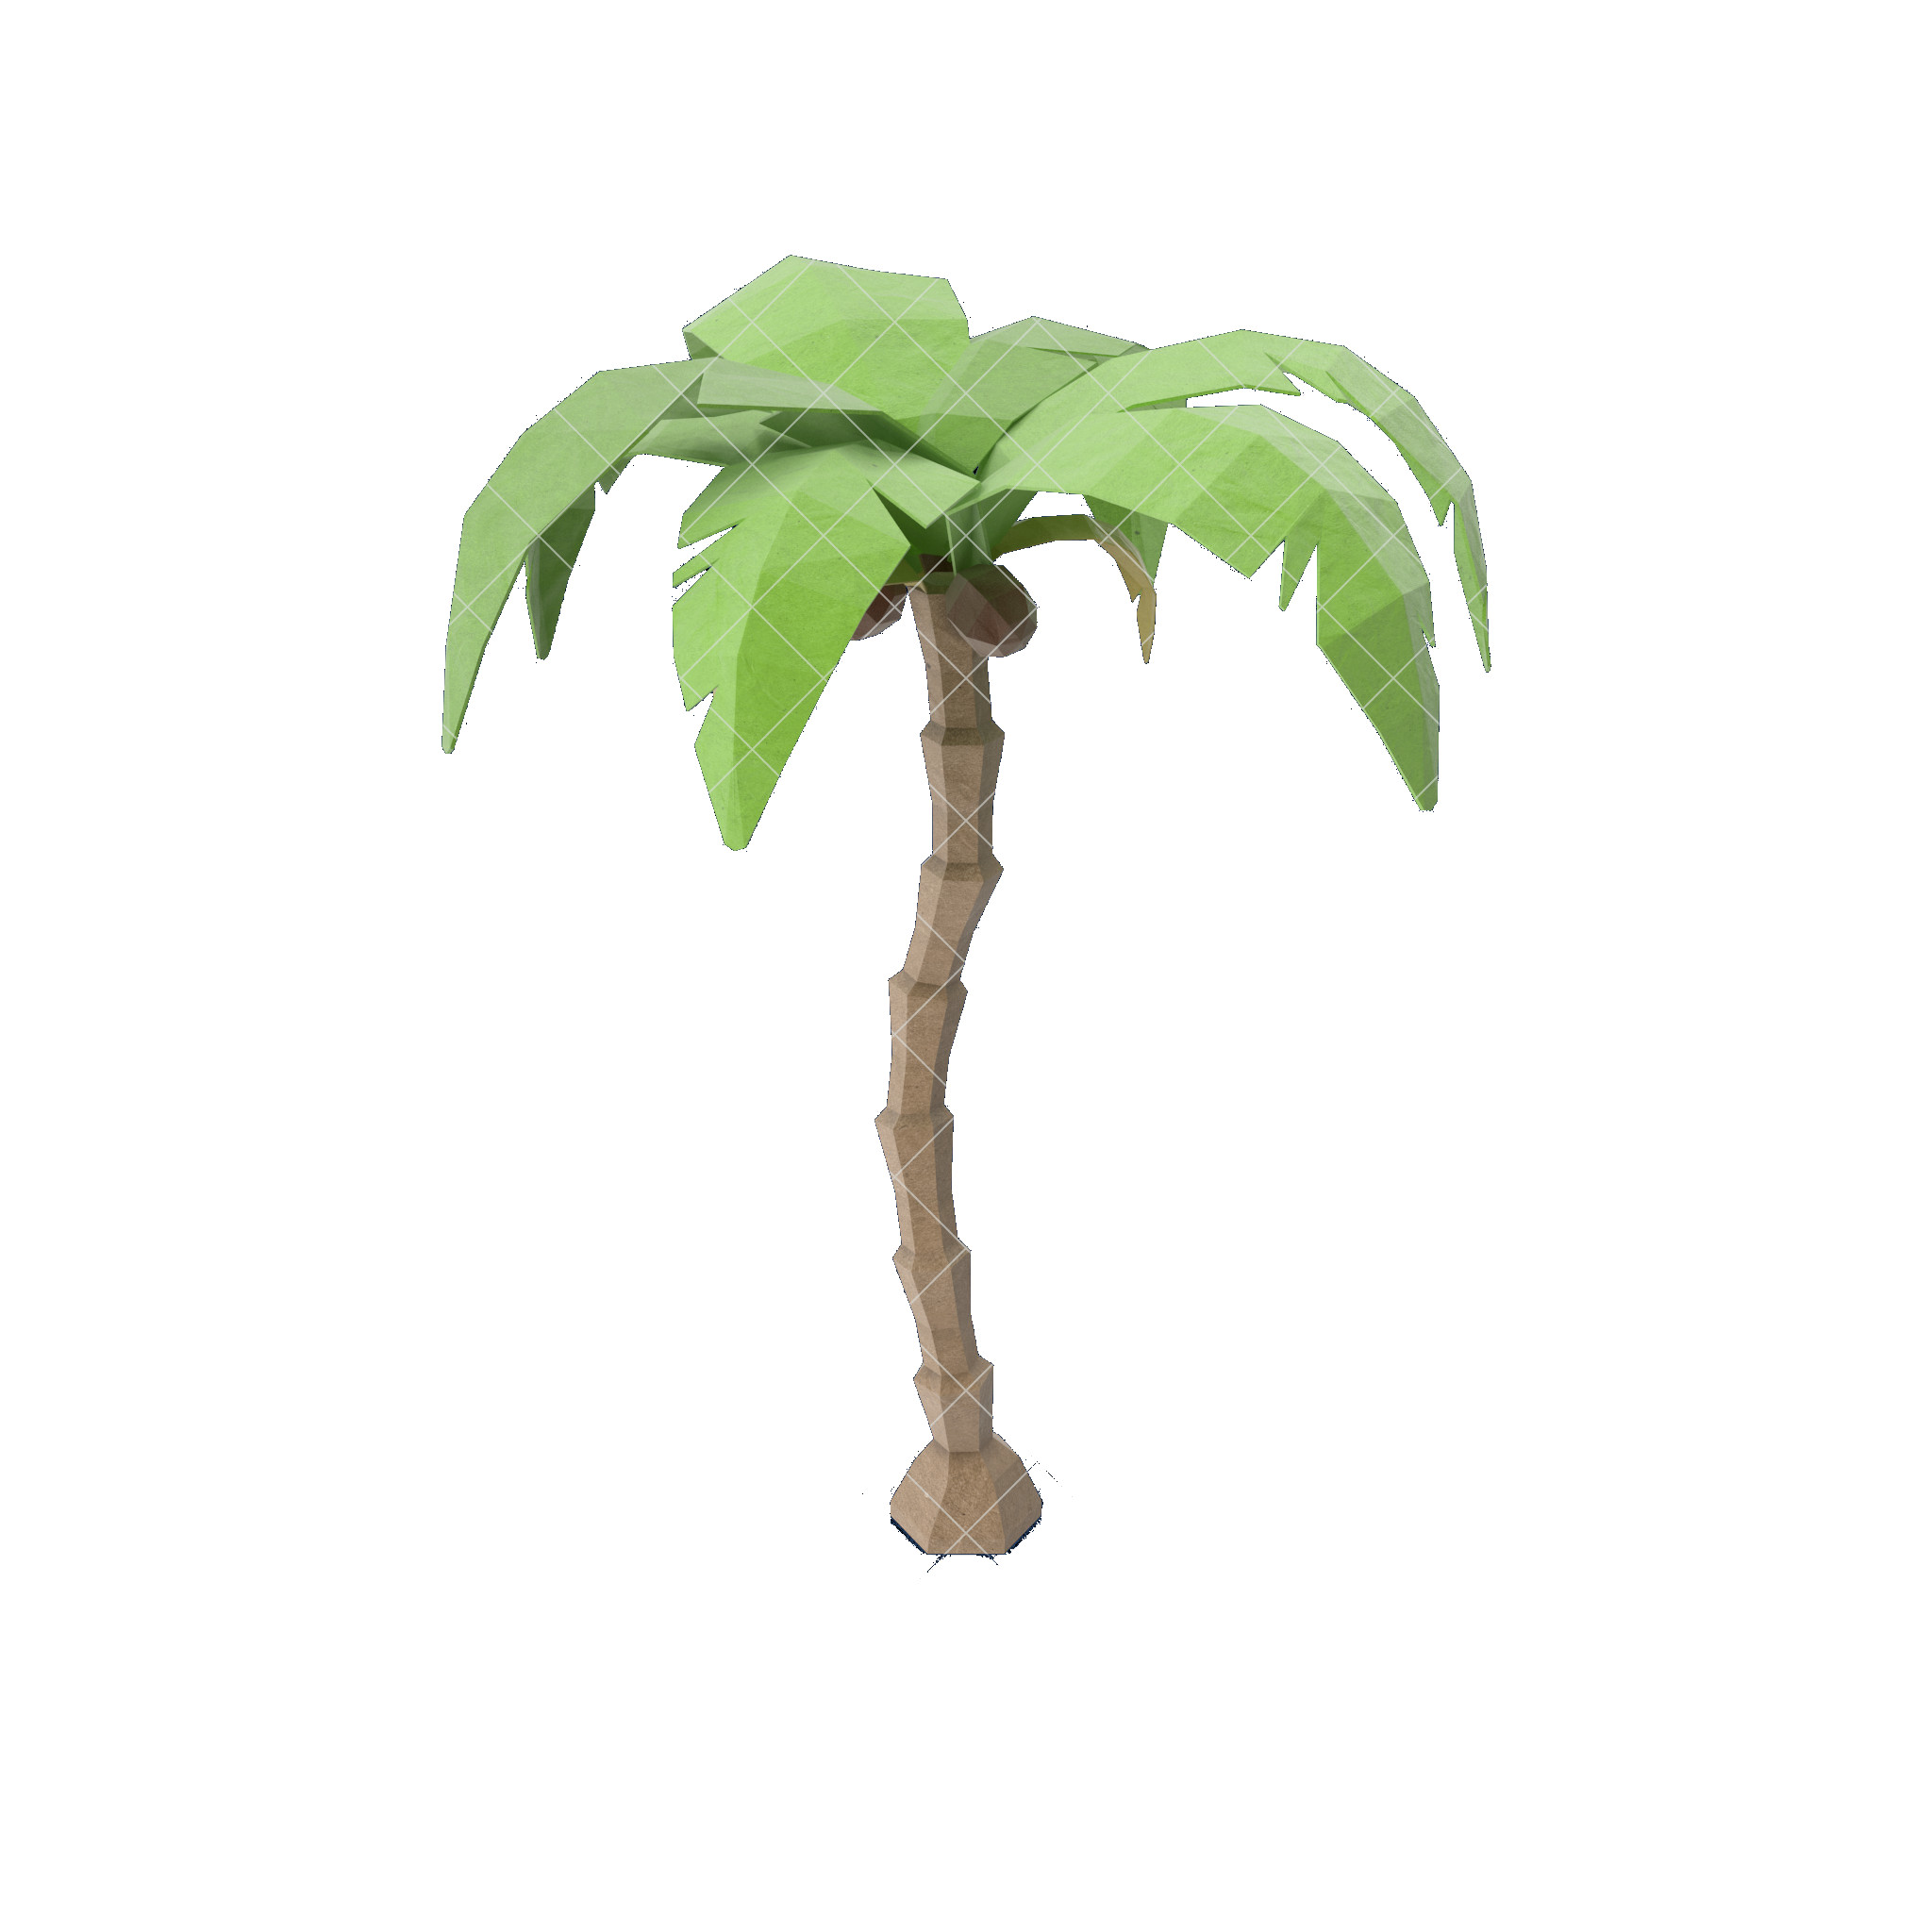
\includegraphics[width=0.6\textwidth]{palmExample}
    \caption{Пример пальмы в стиле low poly. Автор: bgaj23, pixelsquid.com}
    \label{fig:palmExample}
\end{figure}

Для описания формы листьев были использованы квадратичные кривые Безье.  Кривые Безье - это тип кривых, предложенный инженером из компании Renault Пьером Безье в 1962 году. Изначально эти кривые применялись для проектирования кузовов автомобилей, но впоследствии нашли широкое применение в компьютерной графике, где используются для рисования плавных изгибов. На рисунке ~\ref{fig:bezier} дано несколько примеров таких кривых. 

Кривые Безье обладают рядом свойств, благодаря которым они хорошо подходят для использования в компьютерной графике. Их основная ценность заключается в том, что они описываются опорными точками, при перемещении которых кривая изменяется интуитивно понятным образом. Однако кривая Безье не является интерполяцией; как видно по рисунку ~\ref{fig:bezier}, опорные точки не лежат на самой кривой, за исключением первой и последней. 

\begin{figure}[!htb]
    \centering
    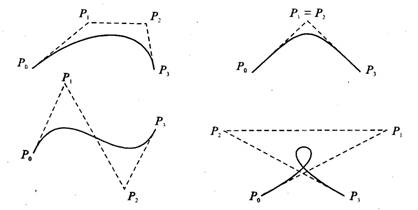
\includegraphics[width=0.6\textwidth]{bezier}
    \caption{Примеры кривых Безье.}
    \label{fig:bezier}
\end{figure}

Кривые Безье задаются рекурсивным выражением, благодаря чему они позволяют описывать сколь угодно сложные кривые. Тем не менее, в целях оптимизации вычислений на практике, как правило, применяются сочетания нескольких кривых небольших порядков. 

Теперь перейдём к формальному определению этого понятия. Кривая Безье порядка $n$ - это плоская полиномиальная кривая, которая задаётся следующим рекурсивным выражением\cite{BezierCurves}:
\begin{equation}
    B_{P_0}(t) = P_0
\end{equation}
\begin{equation*}
    B_{P_{0}...P_{n+1}}(t) = (1 - t) B_{P_{0}...P_{n}}(t) + tB_{P_{1}...P_{n+1}}(t),
\end{equation*}
где \(P_{0}...P_{n}\) - опорные точки. 

Как видно из этого выражения, у квадратичной кривой Безье три опорных точки: $P_0$, $P_1$ и $P_2$. Она имеет форму параболы и определяется следующим выражением:
\begin{equation}
    B(t) = (1 - t)^{2}P_{0} + 2t(1 - t)P_{1} + t^{2}P_{2}
\end{equation}

Таким образом, первая и последняя контрольные точки должны быть размещены в начале и конце листа соответственно, а центральная - посередине со смещением вверх, чтобы регулировать высоту. Это позволит создать лист параболической формы. 

Толщина листа достигает максимума в центре и линейно убывает по мере приближения к концам. Для её вычисления используется формула:
\begin{equation}
    segmentWidth = lerp\left(maxWidth, 0, 2\left|t - \frac{1}{2}\right|\right),
\end{equation}
где $maxWidth$ - заданная в редакторе ширина листа и $t$ - параметр интерполяции, равный 0 в начале листа и 1 в конце.

С заданным шансом на сегментах листа могут появляться треугольные вырезы, символизирующие перистую структуру. При этом сегмент будет состоять не из двух треугольников, как обычно, а из пяти, которые сходятся в одной общей вершине - конце выреза. Вырезы могут появляться на любой стороне сегмента листа или одновременно на обеих. Если на обеих сторонах сегмента появляется вырез, то этот сегмент разделяется надвое отрезком, соединяющим середины его внутренних сторон, и затем вышеописанная операция выполняется с каждой половиной. 

Пример процедурно сгенерированной пальмы показан на рисунке ~\ref{fig:flatResult}.

\begin{figure}[!htb]
    \centering
    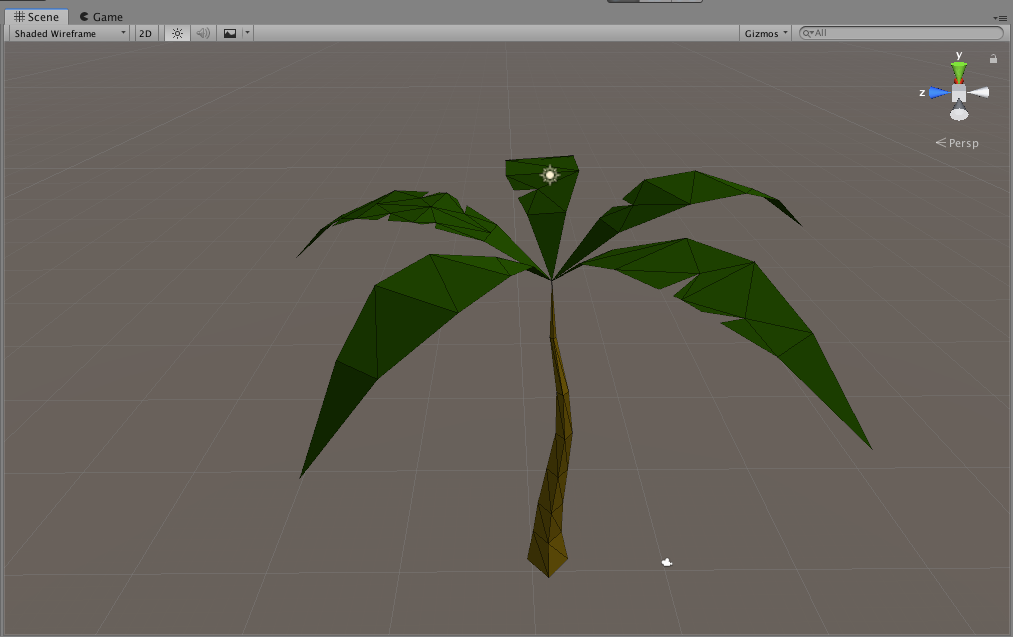
\includegraphics[width=0.6\textwidth]{flatResult}
    \caption{Пример процедурно сгенерированной пальмы.}
    \label{fig:flatResult}
\end{figure}

\section{Генерация хвои}
Последний тип листвы, реализованный в данном плагине - это хвоя. В low poly хвоя состоит из сложенных вертикально пирамид, облегающих ствол и повторяющих его изгибы. Для придания хвое более естественной формы каждую вторую вершину в основании яруса немного сдвигают вниз. На некоторых примерах с рисунка ~\ref{fig:pines} нижний ярус \'уже того, который находится над ним; эта деталь символизирует нижние ветви сосны, отмирающие из-за нехватки солнечного света.  

\begin{figure}[!htb]
    \centering
    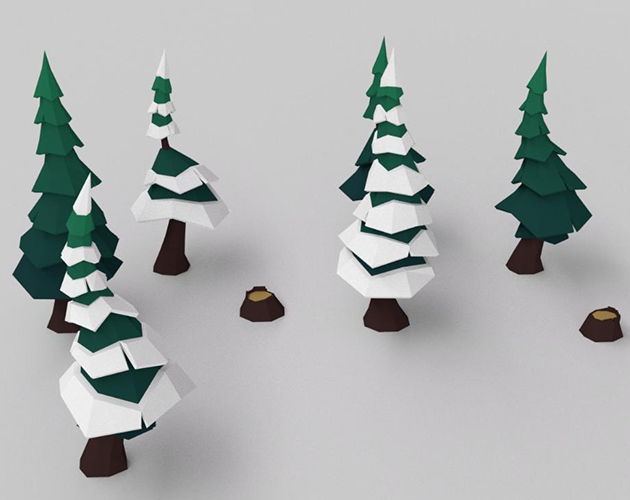
\includegraphics[width=\textwidth]{pines}
    \caption{Сосны в стиле low poly. Автор: TheTeaGuns, itch.io}
    \label{fig:pines}
\end{figure}

В отличие от других типов листвы, хвоя покрывает б\'ольшую часть ствола. По этой причине при генерации ствола необходимо сохранять позицию, поворот и радиус колец ствола, чтобы потом использовать их для генерации хвои. 

Процесс генерации хвои похож на генерацию ствола. Хвоя состоит из ярусов с чередующейся шириной, начинающих покрывать ствол после отступа в несколько сегментов снизу. Внешнее кольцо имеет радиус, равный сумме радиуса ствола и заданного радиуса листвы. Для внутреннего кольца к радиусу ствола прибавляется половина. 

Вначале определяется, будет ли нижний ярус узким. Если он узкий, то его радиус меньше обычного на половину радиуса листвы, а радиус внутреннего кольца яруса, следующего за ним - на четверть. Остальные ярусы генерируются по обычным правилам.

Вершины колец внешнего яруса, индексы которых имеют такую же чётность, что и индексы самого яруса, слегка сдвигаются вниз для придания хвое более естественной формы. Таким образом, на чётных ярусах сдвигаются чётные вершины, а на нечётных - нечётные. 

На рисунке ~\ref{fig:coniferResult} показан пример процедурно сгенерированного дерева с такой листвой. Деревья с хвоей не могут иметь ветви.

\begin{figure}[!htb]
    \centering
    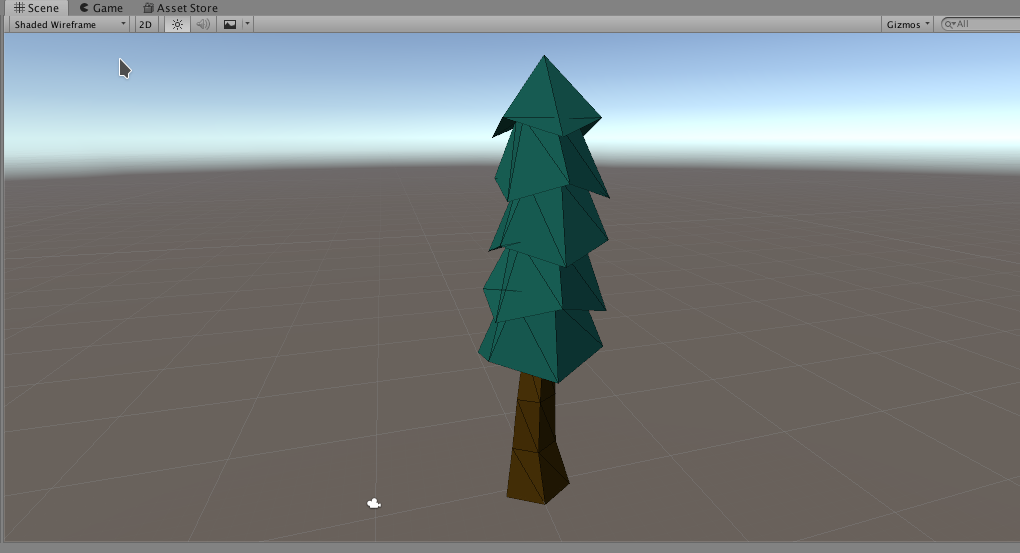
\includegraphics[width=0.8\textwidth]{coniferResult}
    \caption{Пример процедурно сгенерированного хвойного дерева.}
    \label{fig:coniferResult}
\end{figure}

\section{Разработка расширения для редактора}
В данном плагине была реализована возможность генерации различных типов листвы - круглой, плоской и хвои. Для удобной настройки генерации в редакторе должны отображаться только те параметры, которые относятся к выбранному типу листвы. Чтобы решить эту задачу, было создано расширение для редактора.

Стандартный редактор содержит компоненты интерфейса для задания значений общедоступных полей скрипта. Так, для строк используется поле ввода, для булевых значений - переключатель, для цветов - меню выбора цвета и так далее. Для чисел используется ползунок, если с помощью атрибута Range задан диапазон допустимых значений, а в противном случае - поле ввода. 

С помощью атрибутов можно добавить заголовки, изменить отображаемые в редакторе названия полей, скрывать поля из редактора, добавлять всплывающие подсказки и проводить некоторые другие манипуляции. Тем не менее, если этого недостаточно, Unity позволяет создать свой класс редактора для определённого скрипта.

Как и скрипты, расширения для редактора Unity пишутся на языке C\#. Класс расширения редактора должен наследоваться от класса Editor и находиться в одноимённой папке в корне проекта, чтобы Unity мог его зарегистрировать. Для того, чтобы привязать редактор к соответствующему объекту, используется атрибут CustomEditor\cite{UnityEditor}.

Создав своё расширение для редактора, разработчик может манипулировать свойствами редактируемого объекта в сериализованном виде. Сериализация скриптов в Unity нужна для обеспечения работы механизма горячей перезагрузки, благодаря которому редактор сохраняет значения параметров при изменении скрипта. 

Пользовательская логика отображения редактора должна находиться в методе \texttt{OnInspectorGUI}. Сериализованный объект хранится в поле \texttt{serializedObject}, а метод \texttt{FindProperty} позволяет получить доступ к его свойствам. Затем c помощью класса \texttt{EditorGUILayout} выводятся компоненты интерфейса, используемые для изменения значений полей. Наконец, после отрисовки интерфейса необходимо вызвать метод \texttt{serializedObject.ApplyModifiedProperties}, который запишет все изменения из объекта C\# в память.

\begin{figure}[!htb]
    \centering
    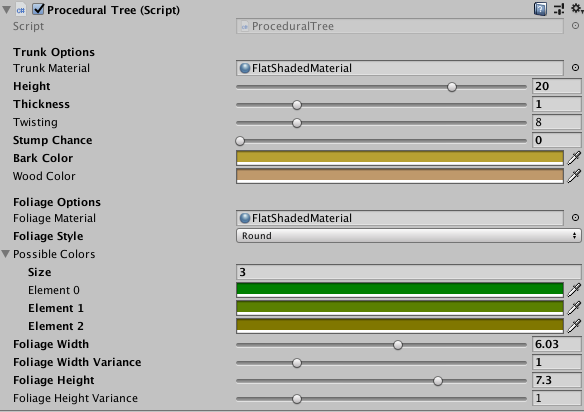
\includegraphics[width=0.8\textwidth]{editor}
    \caption{Интерфейс разработанного расширения редактора.}
\end{figure}

Разработанное расширение позволяет скрывать или отображать  параметры в зависимости от выбранного типа листвы, определяемого полем \texttt{Foliage Style}. Если выбран тип \texttt{None}, то все параметры скрываются, а листва не генерируется.

\newpage

    \chapter{Заключение}
 
В ходе выполнения работы был разработан плагин для движка Unity, позволяющий генерировать low poly модели деревьев во время выполнения. Плагин прост в использовании и подходит для использования в играх для мобильных устройств благодаря простоте результирующих моделей. Поддерживается генерация круглой и плоской листвы, а также хвои. Приведены примеры моделей, созданных в результате работы плагина. Была создана диаграмма классов плагина (рис. ~\ref{classDiagram}), в которую не включены особые настройки типов листвы и поля, используемые для кэширования настроек генерации.

В дальнейшем планируется усовершенствовать алгоритмы генерации для получения более разнообразных и привлекательных моделей, расширить генератор различными типами стволов (например, пальмовый или берёзовый), создать систему пресетов для генерации деревьев на основе предопределённого шаблона, а также улучшить интерфейс редактора.
 
\begin{figure}[h]
    \centering
    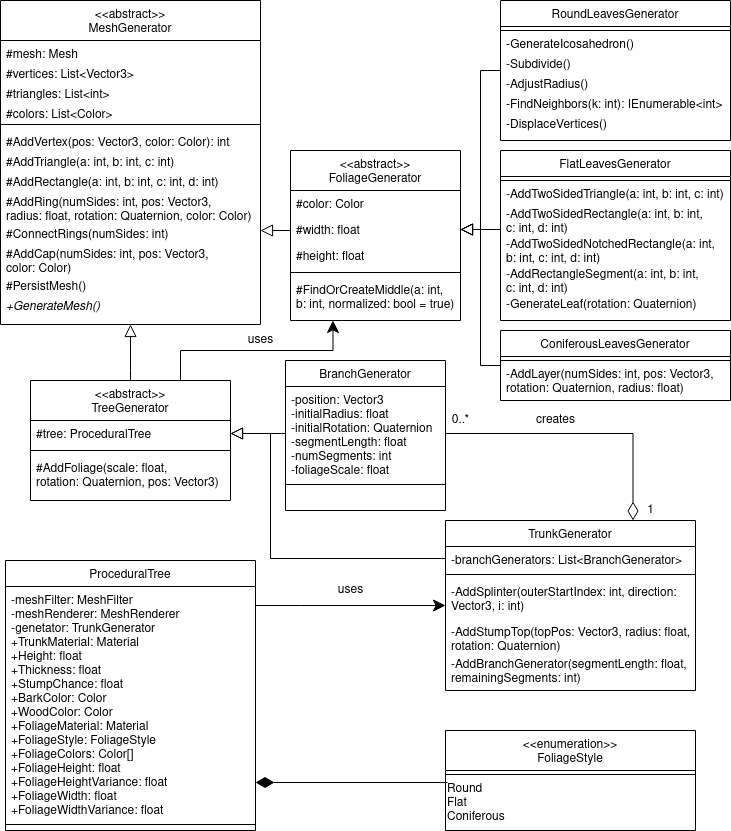
\includegraphics[width=0.8\textwidth]{classDiagram}
    \caption{Диаграмма классов разработанного плагина.}
    \label{classDiagram}
\end{figure}

    
    \addcontentsline{toc}{section}{Список использованных источников}
    \renewcommand\bibname{Список использованных источников}
    
    \begin{thebibliography}{3}
    
    \bibitem{LowPolyIntro}
    An Intro to Low-Poly and Flat Design [Электронный ресурс]. 2018. - URL: https://developer.amazon.com/blogs/appstore/post/aaedd3b8-5e3f-4b4b-a567-c3257139cbcf/an-intro-to-low-poly-and-flat-design;
    
    \bibitem{UnityMesh}
    Unity - Manual: Mesh Components [Электронный ресурс]. URL: https://docs.unity3d.com/Manual/comp-MeshGroup.html;
    
    \bibitem{FlatShader}
    Rendering Flat-Shaded / Low-Poly Style Models in Unity [Электронный ресурс]. 2019. URL: https://hextantstudios.com/unity-flat-low-poly-shader;
    
    \bibitem{IcosahedronMath}
    The Golden Geometry of Solids or Phi in 3 dimensions [Электронный ресурс]. 2016. URL: http://www.maths.surrey.ac.uk/hosted-sites/R.Knott/Fibonacci/phi3DGeom.html;
    
    \bibitem{Subdivision}
    Subdivision of icosahedrons [Электронный ресурс]. 2012. URL: http://blog.coredumping.com/subdivision-of-icosahedrons
    
    \bibitem{BezierCurves}
    Кривые Безье и Пикассо [Электронный ресурс]. 2017. URL: https://habr.com/ru/post/344814/;
    
    \bibitem{hassank}
    Procedural growth of a low poly tree in Unity [Электронный ресурс]. 2016. URL: https://github.com/hassank/TreeGrowth;
    
    \bibitem{friggog}
    Procedural generation of tree models in blender [Электронный ресурс]. 2019. URL: https://github.com/friggog/tree-gen;
    
    \bibitem{treeit}
    Официальный сайт TreeIt [Электронный ресурс]. URL: http://www.evolved-software.com/treeit/treeit;
    
    \bibitem{UnityEditor}
    Unity - Manual: Custom Editors [Электронный ресурс]. URL: https://docs.unity3d.com/Manual/editor-CustomEditors.html;
    
    \bibitem{quaternions}
    Доступно о кватернионах и их преимуществах [Электронный ресурс]. 2018. URL: https://habr.com/ru/post/426863/;
    
    \bibitem{youtube}
    YouTube [Электронный ресурс]. URL: https://youtube.com.
    
    \end{thebibliography}
    
\end{document}
